\documentclass{article}



\usepackage{fullpage}
\usepackage{nopageno}
\usepackage{amsmath}
\usepackage{amsfonts}
\usepackage{graphicx}
\usepackage{framed}
\usepackage{xcolor}

\definecolor{dark_red}{rgb}{0.5,0.0,0.0}
\definecolor{dark_green}{rgb}{0.0,0.5,0.0}
\definecolor{dark_blue}{rgb}{0.0,0.0,0.5}

\newcommand{\dr}[1]{\textcolor{dark_red}{#1}}
\newcommand{\dg}[1]{\textcolor{dark_green}{#1}}
\newcommand{\db}[1]{\textcolor{dark_blue}{#1}}


\begin{document}

Recall that \(\mathbf{i}\) is a vector with a length of \(1\) that points in the direction of the positive \(x\)-axis, and that \(\mathbf{j}\) is a vector with a length of \(1\) that points in the direction of the positive \(y\)-axis. An arbitrary vector \(\mathbf{v} = \langle v_x, v_y\rangle\) is the sum of its horizontal component \(v_x\mathbf{i}\) and its vertical component \(v_y\mathbf{j}\):
\[\mathbf{v} = \langle v_x, v_y\rangle = v_x\mathbf{i} + v_y\mathbf{j}\] 


\section*{Component vector addition}

\begin{tabular}{cc}
\parbox{0.5\textwidth}{
A major benefit of vectors expressed using component form is that the addition and scalar multiplication of vectors is a trivial matter. Consider two vectors \(\mathbf{u} = \langle u_x, u_y \rangle\) and \(\mathbf{v} = \langle v_x, v_y \rangle\). Adding vectors \(\mathbf{u}\) and \(\mathbf{v}\), as seen in the image on the right, involves adding the horizontal components of \(\mathbf{u}\) and \(\mathbf{v}\) to get the horizontal component of \(\mathbf{u} + \mathbf{v}\); and adding the vertical components of \(\mathbf{u}\) and \(\mathbf{v}\) to get the vertical component of \(\mathbf{u} + \mathbf{v}\). The horizontal component of \(\mathbf{u} + \mathbf{v}\) is \(u_x\mathbf{i} + v_x\mathbf{i} = (u_x + v_x)\mathbf{i}\). The vertical component of \(\mathbf{u} + \mathbf{v}\) is \(u_y\mathbf{j} + v_y\mathbf{j} = (u_y + v_y)\mathbf{j}\). Therefore:
\[\mathbf{u} + \mathbf{v} = \langle u_x + v_x, u_y + v_y \rangle\]
Vectors are added by simply adding together their corresponding horizontal and vertical components.
} & \parbox{0.5\textwidth}{
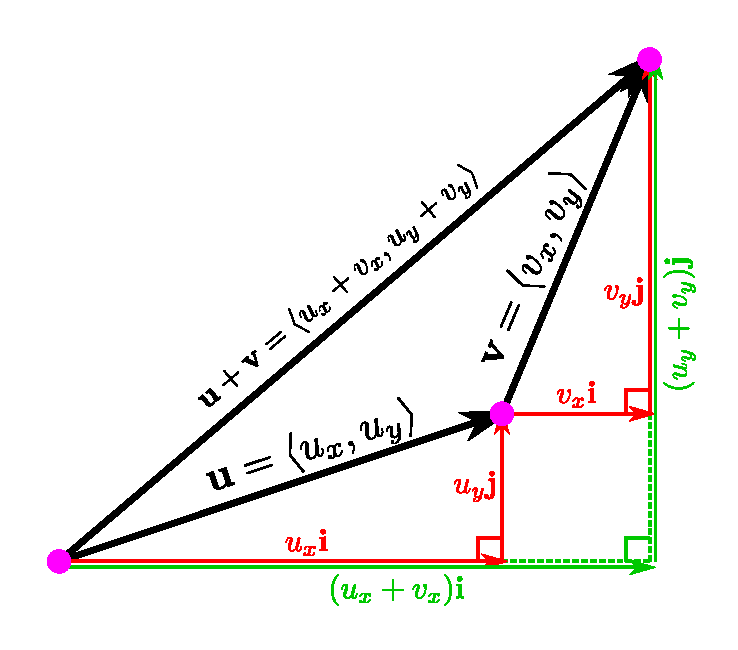
\includegraphics[width = 0.5\textwidth]{component_vector_addition}
}
\end{tabular}

\textbf{Examples:}
\begin{itemize}
\item \(\langle 11, 9 \rangle + \langle -5, -7 \rangle = \langle 11 - 5, 9 - 7 \rangle = \langle 6, 2 \rangle\)
\item \(\langle 34, -24 \rangle + \langle 23, 41 \rangle = \langle 34 + 23, -24 + 41 \rangle = \langle 57, 17 \rangle\)
\item \(\langle 2, -24 \rangle + \langle 18, 21 \rangle = \langle 2 + 18, -24 + 21 \rangle = \langle 20, -3 \rangle\)
\end{itemize}


\section*{Component vector negatives}

\begin{tabular}{cc}
\parbox{0.5\textwidth}{
The negative of a vector \(\mathbf{v} = \langle v_x, v_y \rangle\) is determined by simply reversing the direction of \(\mathbf{v}\). In terms of components, the sign of each component is flipped:
\[-\mathbf{v} = \langle -v_x, -v_y \rangle\]
When a vector \(\mathbf{v}\) is subtracted from a vector \(\mathbf{u}\), what is happening is that the negative of \(\mathbf{v}\) is being added to \(\mathbf{u}\): 
\[\mathbf{u} - \mathbf{v} = \mathbf{u} + (-\mathbf{v})\]
} & \parbox{0.5\textwidth}{
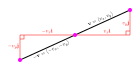
\includegraphics[width = 0.5\textwidth]{component_vector_negative}
}
\end{tabular}
\[\langle u_x, u_y \rangle - \langle v_x, v_y \rangle = \langle u_x, u_y \rangle + \langle -v_x, -v_y \rangle = \langle u_x - v_x, u_y - v_y \rangle\]


\section*{Component vector scalar multiplication}

Consider an arbitrary vector \(\mathbf{v} = \langle v_x, v_y \rangle\). For an arbitrary natural number \(n \in \{1, 2, 3, ...\}\), adding \(n\) copies of \(\mathbf{v}\) together gives \(n\mathbf{v}\):
\begin{align*}
n\mathbf{v} = & \underbrace{\mathbf{v} + \mathbf{v} + \cdots + \mathbf{v}}_n 
= \underbrace{\langle v_x, v_y \rangle + \langle v_x, v_y \rangle + \cdots + \langle v_x, v_y \rangle}_n 
= \left\langle \underbrace{v_x + v_x + \cdots + v_x}_n, \underbrace{v_y + v_y + \cdots + v_y}_n \right\rangle \\  
= & \langle n v_x, n v_y \rangle
\end{align*}
Therefore:
\[n\mathbf{v} = \langle n v_x, n v_y \rangle\]

Generalizing the natural number \(n\) to a real number \(c \in \mathbb{R}\) gives the general formula scalar multiplication:
\[c\mathbf{v} = \langle c v_x, c v_y \rangle\]
In essence, multiplication by a scalar \(c\) simply involves the multiplication of each component by \(c\).

\textbf{Examples:}
\begin{itemize}
\item \(3\langle -1, 5 \rangle = \langle 3 \cdot (-1), 3 \cdot 5 \rangle = \langle -3, 15 \rangle\)
\item \(-2\langle 4, 7 \rangle = \langle (-2) \cdot 4, (-2) \cdot 7 \rangle = \langle -8, -14 \rangle\)
\item \(5\langle 0.2, -1.2 \rangle = \langle 5 \cdot (0.2), 5 \cdot (-1.2) \rangle = \langle 1, -6 \rangle\)
\end{itemize}


\section*{Component vector magnitude}

\begin{tabular}{cc}
\parbox{0.5\textwidth}{
Consider an arbitrary vector \(\mathbf{v} = \langle v_x, v_y \rangle\). Through use of the Pythagorean theorem, the length (or magnitude) of \(\mathbf{v}\), denoted by \(\|\mathbf{v}\|\), satisfies \(\|\mathbf{v}\|^2 = |v_x|^2 + |v_y|^2\). Therefore:
\[\|\mathbf{v}\| = \sqrt{v_x^2 + v_y^2}\]
} & \parbox{0.5\textwidth}{
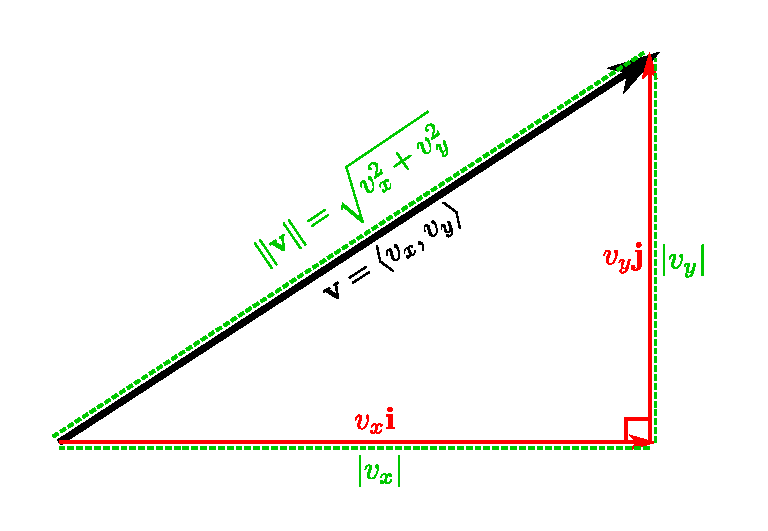
\includegraphics[width = 0.5\textwidth]{component_vector_magnitude}
}
\end{tabular}

\textbf{Examples:}
\begin{itemize}
\item \(\|\langle -3, 4 \rangle\| = \sqrt{(-3)^2 + 4^2} = \sqrt{9 + 16} = \sqrt{25} = 5\)
\item \(\|\langle 12, -5 \rangle\| = \sqrt{12^2 + (-5)^2} = \sqrt{144 + 25} = \sqrt{169} = 13\)
\item \(\|\langle -3, -1 \rangle\| = \sqrt{(-3)^2 + (-1)^2} = \sqrt{9 + 1} = \sqrt{10} \approx 3.16228\)
\end{itemize}


\section*{Putting it all together}

\begin{itemize}
\item \(6\langle 2, -3 \rangle - \langle -5, 7 \rangle = \langle 12, -18 \rangle + \langle 5, -7 \rangle = \langle 17, -25 \rangle\)
\item \(\|\langle 3, 2 \rangle + 2\langle 1.5, -0.5 \rangle\| = \|\langle 3, 2 \rangle + \langle 3, -1 \rangle\| = \|\langle 6, 1 \rangle\| = \sqrt{6^2 + 1^2} = \sqrt{37} \approx 6.08276\)
\end{itemize}

\end{document}











